\chapter{\sffamily Dynamic spatial fields}

{\bfseries\sffamily Concept.} To define and develop an archetype simulation environment for dynamic spatial fields. In our classification scheme, this archetype is defined by a highly-structured, totally connected, bidirectional state partition graph topology and would make sense for simulations of spatial epidemiological processes, ecosystems and weather. We will also discuss the typical ways in which the spatial state partitions of the system may only partially be observed in realistic examples, and analyse how best to deal with each situation. For the mathematically-inclined, this chapter will define the mapping of our formalism to dynamic spatial fields. For the programmers, the software which is designed and described in this chapter can be found in the public Git respository here: \href{https://github.com/worldsoop/worldsoop}{https://github.com/worldsoop/worldsoop}.


\section{\sffamily Defining the archetype}

The dynamic spatial field archetype refers to simulation environments which have highly-structured, bidirectional communication between state partitions. The graph toplogy of this archetype is totally connected, but some connections matter more than others. As a helpful analogy, you can think of these partitions as being structured topologically in a kind of `lattice' configuration, where connections to other partitions over different distances in the lattice can contribute different importance weights in affecting each local state partition. This lattice structure can be best intuited from a visual discription, so we have illustrated an example graph topology for the dynamic spatial field archetype in Fig.~\ref{fig:state-partition-graph-dynamic-spatial-fields}.

\begin{figure}[h]
\centering
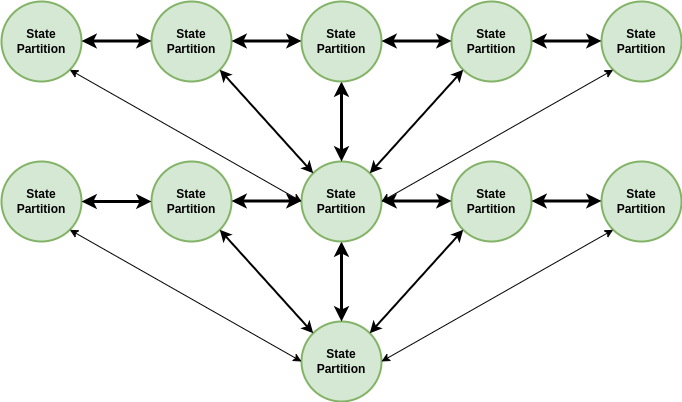
\includegraphics[width=11cm]{images/chapter-7-state-partition-graph.drawio.png}
\caption{State partition graph topology for dynamic spatial field archetypes. The graph should be totally connected but we only show some of the possible connections for simplicity.}
\label{fig:state-partition-graph-dynamic-spatial-fields}
\end{figure}

Depending on the spatial dimensionality of the field, we might need to visualise the lattice in Fig.~\ref{fig:state-partition-graph-dynamic-spatial-fields} as existing in more spatial dimensions than the 2-dimensional example we have illustrated. However, as it turns out, there are many important real-world examples of 2-dimensional spatial systems to control anyway. 

Before we move onto a discussion of data, we can study spatial systems which follow this archetype a little more mathematically by adapting the probabilistic formalism we developed in the first part of this book. 

\textcolor{red}{Need to give more recall to the reader here about the probabilistic formalism...}

Let's return to this probabilistic formalism that we introduced earlier and note that the covariance matrix estimate with elements $C^{ij}_{{\sf t}+1}(z)$ represents a matrix that could get very large, depending on the problem. For example; if we encoded the state of a 2-dimensional spatial field of values into the elements $X^i_{\sf t}$, the number of elements in the covariance matrix $C^{ij}_{{\sf t}+1}(z)$ would scale as $4N^2$ --- where $N$ here is the number of spatial points we wanted to encode. 

One solution to this scaling problem is to exploit the fact that, in many spatial processes, the proximity of points can strongly determine how correlated they are. Hence, for pairwise distances further than some threshold, the covariance matrix elements should tend towards 0. If we were to place points along the diagonal of $C^{ij}_{{\sf t}+1}(z)$ in order of how close they are to each other, this threshold would then be represented as a \emph{banded matrix}. We have illustrated such a matrix in Fig.~\ref{fig:banded-matrix} in which the `bandwidth' is defined as the number of diagonals one needs to traverse from the main diagonal before encountering a diagonal of 0s.

\begin{figure}[h]
\centering
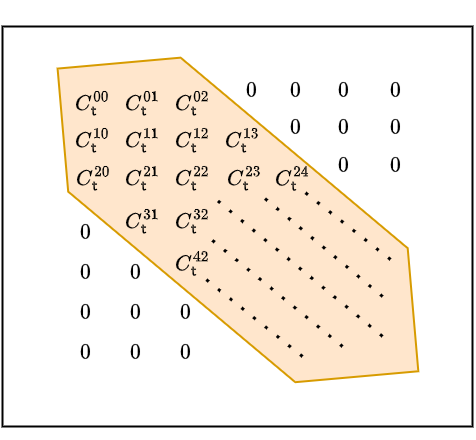
\includegraphics[width=9cm]{images/chapter-7-banded-matrix.drawio.png}
\caption{An illustration of a banded covariance matrix with a bandwidth of 2.}
\label{fig:banded-matrix}
\end{figure}

\textcolor{red}{
\begin{itemize}
\item{At some point it might be sensible to move into the Fourier domain here --- at least for derivations and calculations. Probably more intuitive for the reader to keep it mostly in real space though if possible.} 
\item{The extra detail that's also needed here is to consider how we encode a 2-dimensional spatial process into our state vector, and how the elements of the resulting state vector might be correlated to one another depending on their spatial proximity. If we start with a Markovian Gaussian random field, we can derive the Mat\'{e}rn kernel over these spatial coordinates in order to correlate the state vectors in such a way.} 
\item{Also look into the Radial Basis Function (RBF) and higher-order derived kernels based on DALI expansion~\cite{sellentin2014breaking} in order to try and capture non-Gaussianity.}
\end{itemize}
}

To begin our discussion of data, let's start by considering the subset of real-world problem domains which best suit the dynamic spatial field archetype. These would be:
%%
\begin{itemize}
\item{Spatial simulations of population disease spread and control in the context of global disease outbreaks~\cite{ohi2020exploring} or endemic, spatially-clustered infections like malaria~\cite{carter2000spatial}.}
\item{Spatial ecosystem management environments to infer forest wildfire dynamics~\cite{ganapathi2018using} or improve conservation decision-making~\cite{lapeyrolerie2022deep}.}
\item{Weather system simulations to improve decision-making for agricultural yields~\cite{chen2021reinforcement} or enhance stormwater flood mitigations~\cite{saliba2020deep}.}
\end{itemize}
%%